\section*{Appendix}

All supporting materials which are too extensive for the body text are included here.

\phantomsection
\label{app:A}
\subsection*{Appendix A: Sample Records and Detailed Annotation Procedure}

\subsubsection*{A.1 Sample-Level Record}

A total of 8{,}816 images were photographed over a 3-day collection period beginning January 2026, at the Bandarawela collecting centre (Section~\ref{sec:m_samples}). After the two-stage quality-control correction described in Section~\ref{sec:annotation_qc} -- re-annotating mismatched defect boxes and removing publicly-sourced defect images with inconsistent capture conditions -- the corrected, currently used dataset comprises 7{,}849 distinct captured images. Table~\ref{tab:appendixA_samples} reproduces the final per-class, per-split instance counts (Table~\ref{tab:instances} in the main text).

\begin{table}[H]
\caption{Final per-class annotated instance counts by dataset split}
\label{tab:appendixA_samples}
\centering
\begin{tabular}{lrrrrr}
\toprule
\textbf{Class} & \textbf{Train (cap.)} & \textbf{Train (aug.)} & \textbf{Val.} & \textbf{Test} & \textbf{Total} \\
\midrule
breaker & 1{,}137 & 0   & 326 & 191 & 1{,}654 \\
defect  & 448   & 896 & 137 & 66  & 1{,}547 \\
green   & 1{,}380 & 0   & 429 & 191 & 2{,}000 \\
red     & 1{,}434 & 0   & 395 & 190 & 2{,}019 \\
turning & 1{,}138 & 0   & 309 & 149 & 1{,}596 \\
\midrule
\textbf{Total} & \textbf{5{,}537} & \textbf{896} & \textbf{1{,}596} & \textbf{787} & \textbf{8{,}816} \\
\bottomrule
\end{tabular}
\end{table}

\subsubsection*{A.2 Inclusion and Exclusion Criteria}

\begin{itemize}
    \item Fruit was sourced from a single commercial collecting centre (Bandarawela, Badulla District) so that size, texture, maturity and handling-damage variation reflected normal multi-farm supply rather than a single grower.
    \item Each fruit was pre-sorted by eye at the point of capture into one of the five target categories (green, breaker, turning, red, defect) using the red-surface-percentage criteria in Table~\ref{tab:ripeness}.
    \item Images were captured only inside the lightbox under the fixed lighting arrangement; images captured under any other lighting or background were not added to the training, validation or test pool (Section~\ref{sec:m_sampling}).
    \item Defect images originally sourced from a public dataset were later excluded in full during the quality-control correction of Section~\ref{sec:annotation_qc}, because their background and lighting differed from the project's own captures and had become a misleading cue rather than a genuine signal of damage.
\end{itemize}

\subsubsection*{A.3 Annotation Procedure}

All images were annotated and version-controlled in Roboflow \citep{dwyer2024} and exported in YOLOv8 label format (Section~\ref{sec:m_annotation}). The procedure followed was:

\begin{enumerate}
    \item \textbf{Upload.} Captured images were uploaded in per-session batches.
    \item \textbf{Box drawing.} Every visible fruit in an image was given its own bounding box drawn around the whole fruit. For the defect class specifically, the box covers the entire fruit rather than only the blemished region, so that the model also learns a consistent box scale for every class (Section~\ref{sec:m_annotation}).
    \item \textbf{Class labelling.} Each box was assigned exactly one of the five class labels (breaker, defect, green, red, turning) according to the criteria in Table~\ref{tab:ripeness}.
    \item \textbf{Review.} A second pass reviewed the annotated images and identified two problems that were subsequently corrected (Section~\ref{sec:annotation_qc}): boxes drawn around only the blemish, rather than the whole fruit, on defect images inherited from an external dataset; and defect images whose background and lighting differed from the rest of the dataset. Both were corrected by re-annotation or removal.
    \item \textbf{Export.} The corrected dataset was exported in YOLOv8 format -- one label file per image, each line giving a class index and a normalised box centre, width and height -- and split 70:20:10 into training, validation and test sets (Table~\ref{tab:split}).
\end{enumerate}

\phantomsection
\label{app:B}
\subsection*{Appendix B: Training Configuration, Raw Experimental Records and Shelf Life Data}

\subsubsection*{B.1 Training Configuration for the Deployed Model}

Table~\ref{tab:appendixB_config} lists the full training configuration for the deployed model, expanding on the summary already given in Table~\ref{tab:training}. All values not listed in Table~\ref{tab:training} are standard defaults of the training framework used and were not adjusted for this project.

\begin{table}[H]
\caption{Full training configuration for the deployed model}
\label{tab:appendixB_config}
\centering
\begin{tabularx}{\textwidth}{>{\raggedright\arraybackslash}p{6cm} >{\raggedright\arraybackslash}X}
\toprule
\textbf{Parameter} & \textbf{Value} \\
\midrule
Base architecture & YOLOv8-medium, pre-trained weights \\
Maximum epochs / early-stopping patience & 150 / 25 epochs without improvement \\
Batch size & Selected automatically \\
Input size & 640 $\times$ 640 pixels \\
Initial learning rate / final learning rate factor & 0.01 / 0.01 \\
Momentum / weight decay & 0.937 / 0.0005 \\
Warm-up period & 3 epochs \\
Loss weighting (box / classification / distribution focal) & 7.5 / 0.5 / 1.5 \\
Colour augmentation (hue / saturation / value) & 0.015 / 0.7 / 0.4 \\
Geometric augmentation (rotation / translation / scale) & 15\textdegree\ / 0.1 / 0.5 \\
Flipping & Horizontal only (vertical disabled) \\
Mosaic / mixup augmentation & 1.0 / 0.15 \\
Random erasing & 0.4 \\
Non-maximum-suppression overlap threshold & 0.7 \\
\bottomrule
\end{tabularx}
\end{table}

\subsubsection*{B.2 Per-Epoch Metric Log}

Training ran for 77 logged epochs before early stopping (25 epochs without validation improvement), matching the statement in Section~\ref{sec:r_test}. Table~\ref{tab:appendixB_epochs} reproduces the best epoch (52, the checkpoint restored as the final model) and the last logged epoch, on the validation split.

\begin{table}[H]
\caption{Best and last logged training epochs, validation split (deployed model)}
\label{tab:appendixB_epochs}
\centering
\begin{tabular}{lrrrr}
\toprule
\textbf{Epoch} & \textbf{Precision} & \textbf{Recall} & \textbf{mAP50} & \textbf{mAP50-95} \\
\midrule
52 (best, deployed) & 0.924 & 0.931 & 0.960 & 0.730 \\
77 (last, early-stopped) & 0.930 & 0.940 & 0.965 & 0.706 \\
\bottomrule
\end{tabular}

\vspace{2mm}
{\footnotesize Values are on the \emph{validation} split during training, distinct from the single held-out \emph{test}-split evaluation reported in Table~\ref{tab:testresults}.}
\end{table}



\subsubsection*{B.3 Raw Records for Experiment 3 (Live Classification)}

Two live classification sessions were logged, either side of the imaging-conditions correction of Section~\ref{sec:annotation_qc}; their class-distribution totals are reproduced from Table~\ref{tab:liveclass}. Photographic evidence was retained from both sessions. For the live classification validation trial, a sample of \textit{Padma} 50 green tomatoes was specifically selected and tested on the system rather than testing an even distribution across all ripening stages. Neither session recorded a per-fruit ground-truth label for overall class-mix accuracy, so, as stated in Section~\ref{sec:r_live}, no overall percentage accuracy can be derived from this record beyond tracking the distribution shift.



\subsubsection*{B.4 Raw Records for Experiment 4 (Conveyor Transport and Sorting)}

\textbf{Mechanical transport (completed).} A bench trial confirmed smooth, stable belt transport of fresh fruit with no vision or sorting logic active.

\textbf{Closed-loop end-to-end sorting (completed).} The complete pipeline was run against fruit moving on the belt, with the vision system driving the gates through the controller. The system successfully executed the full sequence end to end: each fruit was detected and classified in real time, commands were transmitted to the controller, staged in per-gate queues, and assigned gates opened at speed-scaled intervals after the fruit reached each gate's infrared sensor. All four ripening classes were diverted at their respective gates, and defective fruit passed uninterrupted to the reject stream without lost or duplicated commands.

\subsubsection*{B.5 Shelf-Life Observation Data}

The per-class remaining shelf-life values used by the deployed software, listed in Table~\ref{tab:shelfresults}, are green 31 days, breaker 29 days, turning 24 days, red 12 days and defect 0 days.

This is the same gap already identified in Section~\ref{sec:r_shelflife}: the values above match \citet{abekoon2024}'s published Padma stage durations exactly once mapped through the four-class correspondence of Table~\ref{tab:merge}, which is more consistent with the published figures having been carried into the project's records than with an independent \textit{Padma} 50 green tomatoes replication. Until the underlying raw record is located, or the 31-day trial is repeated and logged, this table should continue to carry that caveat rather than be presented as confirmed independent measurement.

\phantomsection
\label{app:C}
\subsection*{Appendix C: Pin Assignment, Wiring Diagrams and Component Data}

\textbf{A note on the design described.} Over the course of the project, three successive control designs were built, of which only the third is currently deployed. The first used single-letter commands and no proximity sensing, with gate timing computed from an assumed constant belt speed; this design was later abandoned because timing error accumulated with distance along the belt. The second, an intermediate development version, introduced numbered class commands but relied on a manually typed class rather than the trained detector, and was never tested end-to-end on the physical rig. The third and current design, described in this appendix and in Section~\ref{sec:m_integration}, uses real infrared sensors to trigger gate actuation and adds a sequence-numbered acknowledgement protocol for reliable delivery over a wireless link. This is the version integrated with the vision system and used to produce the results reported in Chapter~\ref{ch:results}.

\subsubsection*{C.1 ESP32 Pin Assignment}

Table~\ref{tab:appendixC_pins} gives the pin assignment of the currently deployed control firmware.

\begin{table}[H]
\caption{ESP32 pin assignment, currently deployed firmware}
\label{tab:appendixC_pins}
\centering
\begin{tabularx}{\textwidth}{>{\raggedright\arraybackslash}p{8cm} >{\raggedright\arraybackslash}X}
\toprule
\textbf{Signal} & \textbf{ESP32 pin} \\
\midrule
Stepper driver step signal & GPIO 25 \\
Stepper driver direction signal & GPIO 26 \\
Belt-speed potentiometer (analogue input) & GPIO 34 \\
Gate servo 1 (class 1 = green, furthest from camera) & GPIO 13 \\
Gate servo 2 (class 2 = breaker) & GPIO 12 \\
Gate servo 3 (class 3 = turning) & GPIO 14 \\
Gate servo 4 (class 4 = red, closest to camera) & GPIO 27 \\
Infrared sensor, position 1 (co-located with gate 4, not gate 1) & GPIO 18 \\
Infrared sensor, position 2 (co-located with gate 3) & GPIO 19 \\
Infrared sensor, position 3 (co-located with gate 2) & GPIO 21 \\
Infrared sensor, position 4 (co-located with gate 1) & GPIO 23 \\
\bottomrule
\end{tabularx}

\vspace{2mm}
{\footnotesize All four infrared inputs use a pulled-up digital input with a 20\,ms software debounce. Servo control uses a 50\,Hz pulse-width signal with a 500--2400\,\textmu s pulse range.}
\end{table}

\textbf{On the position/gate numbering mismatch.} The infrared sensor position numbers and the servo/gate numbers are deliberately mirrored, not matched -- confirmed on the physical rig on 2026-08-15, after an earlier assumption that same-numbered sensors and servos were co-located was found to be incorrect. The confirmed arrangement is: position 1 sits next to gate 4 (class 4, red); position 2 next to gate 3 (turning); position 3 next to gate 2 (breaker); position 4 next to gate 1 (class 1, green). Any wiring diagram or physical rebuild must preserve this mirrored mapping rather than a same-number one.

\subsubsection*{C.2 Physical Layout}

The order of stages along the belt, camera end first, confirmed on the physical rig on 2026-08-15, is: gate 4 (red) $\rightarrow$ gate 3 (turning) $\rightarrow$ gate 2 (breaker) $\rightarrow$ gate 1 (green) -- that is, red closest to the camera and green furthest, matching the order stated in Section~\ref{sec:m_prototype}. This resolves, in the thesis's favour, an inconsistency present in an earlier project note dated 2026-07-23, which stated the opposite order (green closest to camera). That earlier note predates the physical confirmation above and should be treated as superseded.

\textbf{Sensor-to-gate timing.} The firmware does not use a measured physical offset, in centimetres, between a sensor and its gate; instead it waits a configurable time after the sensor fires before opening the gate:

\begin{itemize}
    \item A base post-trigger delay of 2000\,ms at the belt's configured top speed, with a manual fine-tuning offset of $-500$\,ms applied on top, for correcting cases where the computed delay is slightly off in practice.
    \item Speed-adaptive scaling, enabled by default: both the gate-open duration and the post-trigger delay are scaled against the belt's current speed relative to its configured top speed (a slower belt gives a shorter gate-open duration and a longer post-trigger delay), within a bounded range so that a near-stopped belt cannot extend the delay indefinitely.
    \item A default gate-open duration of 2000\,ms at top speed, also speed-scaled.
    \item Gate rest and open angles of 180\textdegree\ and 110\textdegree\ respectively.
\end{itemize}

All of the values above can be changed at run time over a serial connection, without reprogramming the microcontroller (Section~C.4). \textbf{[INFORMATION REQUIRED]} No measured physical distance, in centimetres, between the camera, the sensors and the gates was found; only the time-based values above are available.

\subsubsection*{C.3 Wiring Diagrams}

No drawn wiring diagram or schematic image was found for the deployed design; the separation of power domains is documented only as text, consistent with Table~\ref{tab:hardware}:

\begin{itemize}
    \item \textbf{Motor-driver power domain:} a 24\,V, 5\,A supply feeds the stepper driver only.
    \item \textbf{Logic power domain:} a separate 12\,V, 2\,A supply feeds the microcontroller and logic-level circuitry, isolated from the motor and servo rails so that motor and servo switching noise cannot disturb the control electronics (Section~\ref{sec:m_prototype}).
    \item \textbf{Servo power:} the four gate servos are signal-wire-only from the microcontroller -- powered from a separate 5--6\,V supply rather than the microcontroller's own output pin, which cannot source enough current for four servos and risks resetting the board -- with that supply's ground tied back to the microcontroller's ground so the signal wires share a common reference.
\end{itemize}

\begin{figure}[htbp]
    \centering
    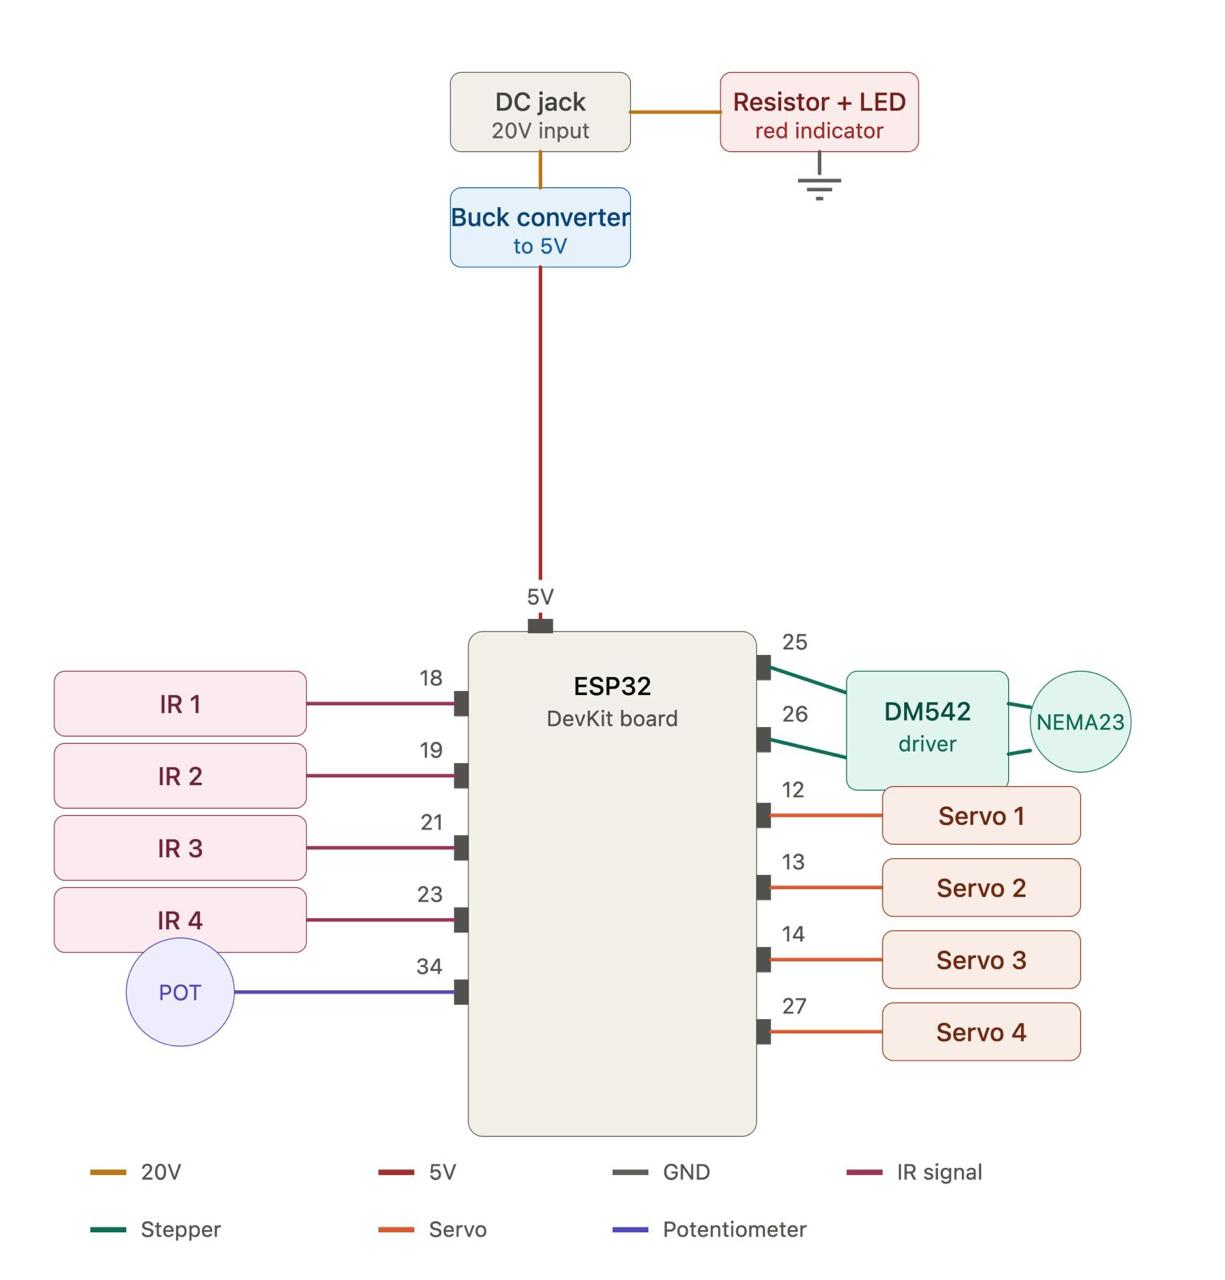
\includegraphics[width=0.95\textwidth]{figures/wiring diagram.jpeg} 
    \caption{Schematic wiring diagram of the ESP32 control system, illustrating GPIO pin configurations, sensor input interfaces, servo/stepper actuator connections, and isolated power distribution domains.}
    \label{fig:wiring_diagram}
\end{figure}

\subsubsection*{C.4 Firmware Logic and Command Protocol}

The firmware is organised into separate modules for the queue-and-gate control logic, the wireless communication link, one module per gate servo, one module per infrared sensor, the belt motor driver, the belt-speed control input, and a single settings module holding every run-time-tunable value.

\textbf{Core decision logic.} Each classified tomato (a value of 1--4, or 0 for no ripeness class) is placed on a queue as soon as it is classified. Every stage of the belt -- there are four, one per gate -- is checked on every control-loop pass: if that stage's sensor has just detected an arriving tomato, the front item is removed from that stage's queue. If the removed class matches the class handled by that stage, the corresponding gate is scheduled to open after the post-trigger delay described in Appendix~C.2, allowing time for the tomato to travel from the sensor to the gate. If the removed class does not match, and the stage is not the last one, the item is placed on the next stage's queue instead, so that it continues to be tracked until it reaches its own gate. There is no per-tomato identity beyond this queue position: correctness depends on classifications being sent, in the same order the tomatoes physically enter the belt, before each tomato reaches the first sensor.

\textbf{Command protocol.} Commands are sent as short text messages, over either a wired or a wireless serial connection, using the same handling either way. Table~\ref{tab:appendixC_protocol} lists the commands understood by the firmware.

\begin{table}[H]
\caption{Command protocol of the currently deployed firmware}
\label{tab:appendixC_protocol}
\centering
\begin{tabularx}{\textwidth}{>{\raggedright\arraybackslash}p{6.5cm} >{\raggedright\arraybackslash}X}
\toprule
\textbf{Command} & \textbf{Effect} \\
\midrule
Class 1--4 (with an optional sequence number) & Places that class on the queue \\
No-class (with an optional sequence number) & Places a ``no gate action'' marker on the queue \\
Reset (with an optional sequence number) & Empties every stage's queue and clears any gate waiting to open \\
Set angles & Sets all four servo angles directly \\
Trigger gate(s) & Opens and returns the listed gate or gates once, for bench testing \\
Set a configuration value & Changes a run-time setting (for example a servo angle, a gate timing value, or the belt speed range) without reprogramming the microcontroller \\
Report motor speed & Returns the belt speed currently commanded by the speed-control input \\
\bottomrule
\end{tabularx}
\end{table}

\textbf{Reliability protocol (sequence number, acknowledgement and retry).} The commands that place an item on a queue -- the four class commands, the no-class command, and reset -- may carry an optional, increasing sequence number. The firmware replies with an acknowledgement that includes the same sequence number and a description of the resulting queue state for every stage. If the same sequence number is received a second time, this is treated as a resend caused by a lost acknowledgement rather than a new command: the firmware repeats the acknowledgement but does not place the tomato on the queue a second time. Reports that the firmware sends on its own initiative, whenever a sensor changes the queue state without being asked, are tagged separately from acknowledgements and carry no sequence number, so that the receiving side can never mistake an unprompted report for a reply to a command it sent. As currently used, the vision and control software sends class commands without a sequence number, relying on the wireless link's own reliability; the sequence-number and acknowledgement mechanism described above is implemented and working in the firmware and can be connected to a retry mechanism on the software side as a contained addition, should stricter delivery confirmation be required for the closed-loop trial noted in Appendix~B.4.

\textbf{Verification.} The firmware was confirmed to build without error and was exercised manually, issuing each command type over a serial connection and confirming the expected servo, sensor and queue-state behaviour, before being connected to the vision system.

\clearpage